% Chapter 4

\chapter{Ensayos y resultados} % Main chapter title

\label{Chapter4}

En el presente capítulo se documenta la evaluación del modelo de detección y del sistema integrado. Se describe el plan de ensayos, se reportan las métricas de reconstrucción y de clasificación sobre escenarios con anomalías conocidas, se analizan los errores cometidos y se registran las pruebas de integración extremo a extremo.

%----------------------------------------------------------------------------------------
%	SECTION 1
%----------------------------------------------------------------------------------------

\section{Plan de evaluación}
\label{sec:plan-evaluacion}

El carácter no supervisado del entrenamiento condicionó la metodología de evaluación. El modelo aprendió a reconstruir el régimen nominal del servicio sin recibir etiquetas de anomalía, de modo que la calidad del aprendizaje y la capacidad de detección se midieron en dos planos complementarios, ya anticipados en la sección~\ref{sec:metricas-evaluacion}.

El primer plano valoró la calidad de reconstrucción sobre tramos considerados nominales mediante el error cuadrático medio (MSE), que cumple el doble papel de función de pérdida y señal escalar de anomalía. El segundo plano valoró la capacidad de detección como un problema de clasificación binaria sobre escenarios controlados con anomalías conocidas, condición necesaria para calcular precisión, sensibilidad, F1-score y tasa de falsos positivos (TFP).

\subsection{Conjuntos de datos y partición}

El entrenamiento utilizó el historial de 90~días descrito en el capítulo~\ref{Chapter3}, particionado en 80~\% para ajuste y 20~\% final para validación, con preservación del orden cronológico para evitar filtraciones de información futura. Ese conjunto de validación cumplió dos funciones: guiar la parada temprana y proporcionar la distribución de errores sobre la que se calibró el umbral de detección.

Para la evaluación de clasificación se construyó un conjunto de prueba independiente de 24~horas, generado por el mismo núcleo de simulación que el servicio simulado (\path{traffic\_simulation\_core.py}) pero con una semilla distinta de la del entrenamiento, de modo que no compartiera realizaciones concretas de ruido con los datos de ajuste. Sobre ese conjunto se inyectaron tres ventanas de anomalía con instantes y duraciones conocidas, listadas en la tabla~\ref{tab:anomalias-inyectadas}. Cada ventana deslizante de prueba se etiquetó como anómala cuando contuvo al menos un instante perteneciente a un tramo inyectado.

\begin{table}[h]
\centering
\small
\caption{Anomalías inyectadas en el conjunto de prueba de 24~horas.}
\label{tab:anomalias-inyectadas}
\begin{tabular}{@{}>{\raggedright\arraybackslash}p{0.24\textwidth}cp{0.46\textwidth}@{}}
\toprule
\textbf{Tipo} & \textbf{Duración} & \textbf{Efecto principal sobre las métricas} \\
\midrule
Pico de latencia & 30~min & Latencia percentil 95 de 2 a 10~s y mayor consumo de CPU \\
Caída de tráfico & 15~min & Tasa de peticiones reducida al 10~\% de la esperada \\
Pico de memoria & 60~min & Memoria residente de 3 a 4~GB y mayor consumo de CPU \\
\bottomrule
\end{tabular}
\end{table}

La elección de tres tipos heterogéneos (incremento sostenido, caída abrupta y consumo anómalo de recursos) buscó cubrir formas distintas de degradación: una de cola superior de latencia, una de descenso de demanda y una de presión de recursos. Esa diversidad permitió analizar no solo el desempeño agregado, sino también el comportamiento del detector frente a anomalías de distinta naturaleza.

\subsection{Confidencialidad de los resultados}

En coherencia con lo expuesto en la sección~\ref{sec:datasets}, los resultados cuantitativos de este capítulo se obtuvieron sobre el entorno demostrativo reproducible, dado que la telemetría productiva es confidencial y no puede publicarse. La validación sobre datos reales se realizó dentro de la infraestructura autorizada de la empresa y se reporta de forma cualitativa, sin exponer series identificables. Las figuras y tablas de desempeño numérico corresponden, por tanto, al conjunto sintético con anomalías inyectadas, que comparte la familia de métricas y la semántica de agregación PromQL del entorno productivo.

\subsection{Métricas y condiciones de prueba}

Las métricas empleadas fueron las definidas en la sección~\ref{sec:metricas-evaluacion}. En el plano de reconstrucción se reportó el MSE de validación. En el plano de clasificación se reportaron exactitud, precisión, sensibilidad, F1-score y tasa de falsos positivos, junto con la matriz de confusión. Todas las pruebas se ejecutaron en CPU, con el mismo par modelo--preprocesador y el mismo umbral serializado que se utilizan en producción, de modo que la evaluación reflejara el comportamiento real de inferencia y no una configuración optimizada solo para el ensayo.

El procedimiento se automatizó en el script \path{scripts/evaluate\_model.py}, que generó el conjunto de prueba, cargó los artefactos, calculó los errores de reconstrucción, clasificó cada ventana respecto del umbral y produjo las visualizaciones. Los resultados iterativos se registraron en \path{evaluation/evaluation\_iterations.csv}. Un barrido de umbrales sobre percentiles del error en tramos nominales permitió analizar el compromiso entre sensibilidad y falsos positivos sin reentrenar el modelo.

%----------------------------------------------------------------------------------------
%	SECTION 2
%----------------------------------------------------------------------------------------

\section{Evaluación del modelo}
\label{sec:evaluacion-modelo}

Los resultados del entrenamiento y del conjunto de prueba con anomalías inyectadas se organizan en torno a dos ejes: la calidad de reconstrucción sobre tramos nominales y la capacidad de clasificación binaria con el umbral calibrado. A continuación se reportan ambos planos, el contraste visual entre ventanas nominales y anómalas, la sensibilidad al umbral, la comparación con una línea base de umbrales fijos y la latencia de detección por tipo de perturbación.

\subsection{Calidad de reconstrucción}

El entrenamiento convergió de forma estable. La pérdida de entrenamiento descendió hasta el orden de $1{,}4\times10^{-3}$ y la pérdida de validación se estabilizó en torno a $3\times10^{-4}$ en la escala normalizada, sin signos de sobreajuste tras la activación de la parada temprana. Sobre los tramos nominales del conjunto de prueba, el error de reconstrucción se concentró en valores bajos: el percentil 95 quedó cerca de $6\times10^{-4}$ y el percentil 99 cerca de $1{,}7\times10^{-3}$, por debajo del umbral calibrado de $0{,}0025$. Las ventanas anómalas, en cambio, alcanzaron errores de hasta dos órdenes de magnitud mayores. Ese margen entre el error típico del régimen nominal y el umbral es el que sostiene una baja tasa de falsas alertas sobre comportamiento habitual.

La figura~\ref{fig:eval-modelo} resume la evaluación en cuatro paneles. El panel superior izquierdo muestra la distribución del error de reconstrucción para ventanas nominales y anómalas: las primeras se concentran en valores bajos, a la izquierda del umbral, mientras que las segundas se desplazan hacia errores marcadamente mayores. Esa separación entre ambas poblaciones es la propiedad que hace viable la detección por umbral sobre una única señal escalar.

\begin{figure}[h]
\centering
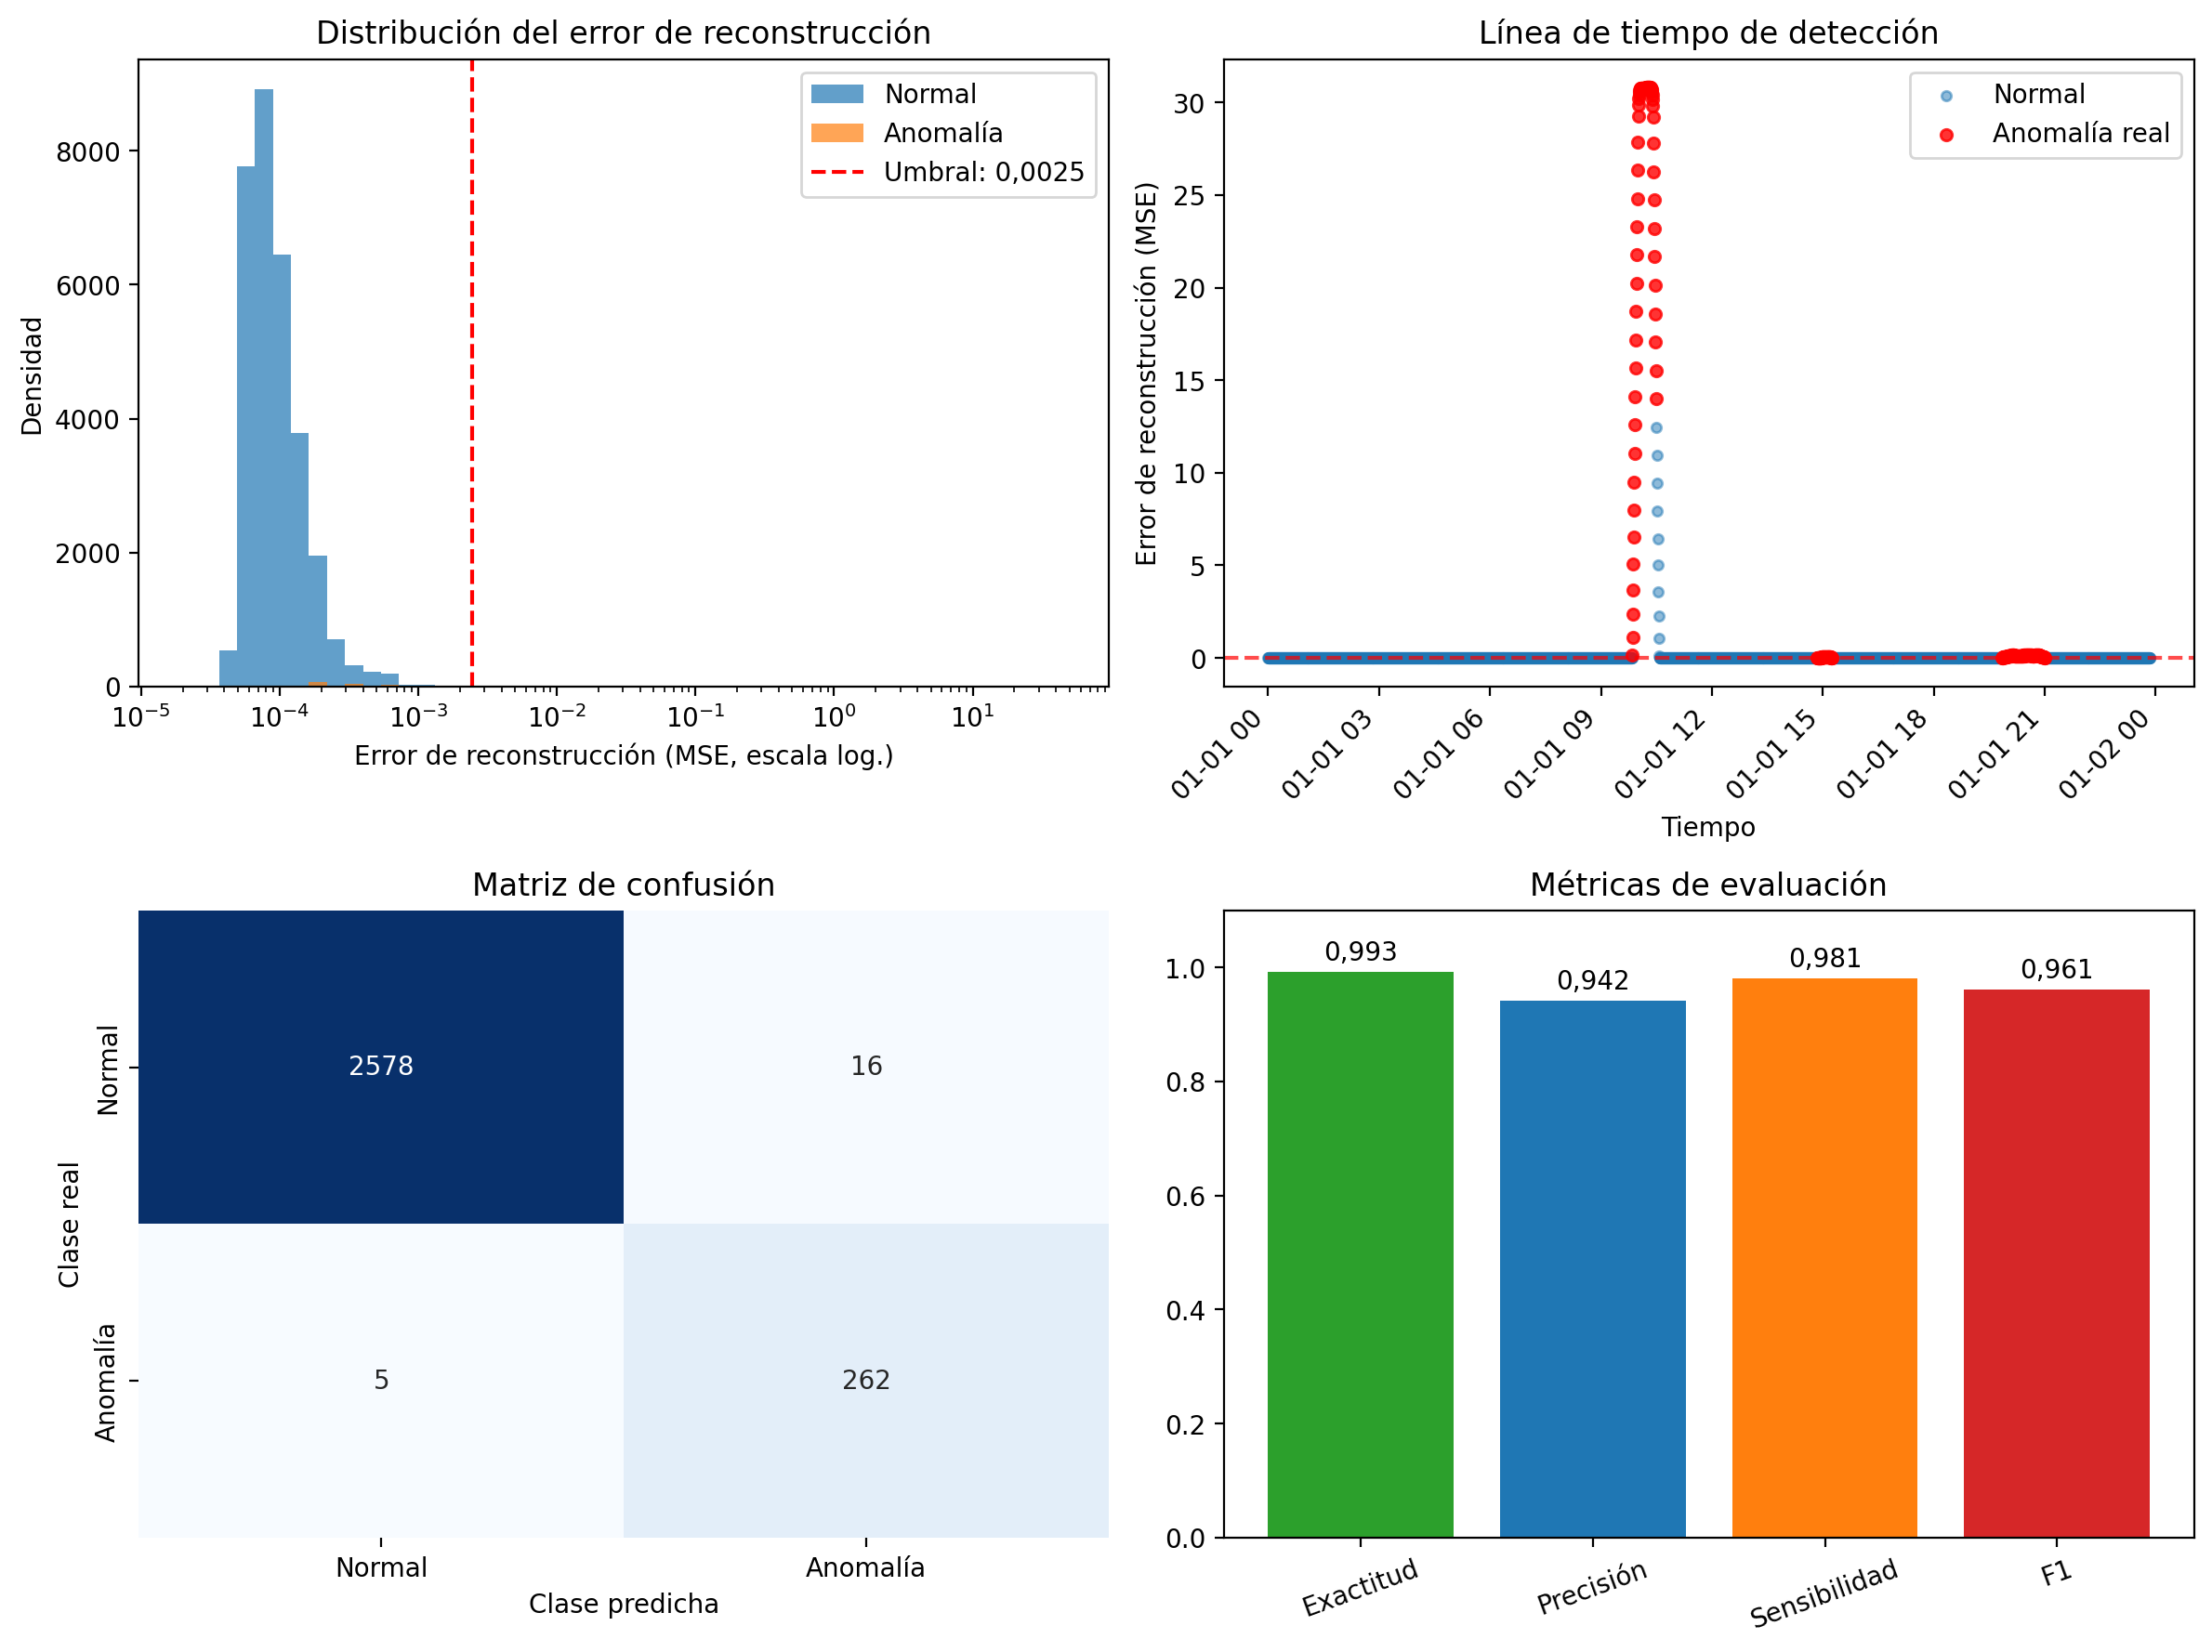
\includegraphics[width=0.95\textwidth]{./Figures/evaluacion_modelo.png}
\caption{Evaluación del modelo sobre el conjunto de prueba con anomalías inyectadas: distribución del error, línea de tiempo de detección, matriz de confusión y métricas.}
\label{fig:eval-modelo}
\end{figure}

\subsection{Reconstrucción de ventanas nominales y anómalas}

Para ilustrar el mecanismo de detección, la figura~\ref{fig:reconstruccion} compara la señal observada y su reconstrucción en dos ventanas concretas del conjunto de prueba. En la ventana nominal del panel izquierdo, la reconstrucción sigue de cerca a cada métrica observada y el error resultante es muy bajo. En la ventana correspondiente al pico de latencia del panel derecho, la latencia percentil 95 observada se elevó muy por encima del régimen nominal aprendido, mientras que la reconstrucción la mantuvo en valores habituales. Esa discrepancia elevó el error de reconstrucción varios órdenes de magnitud respecto del umbral. El contraste confirma que el autoencoder no copia la entrada, sino que la proyecta sobre el comportamiento nominal comprimido en el espacio latente: un patrón ausente del entrenamiento se traduce en un error elevado.

\begin{figure}[h]
\centering
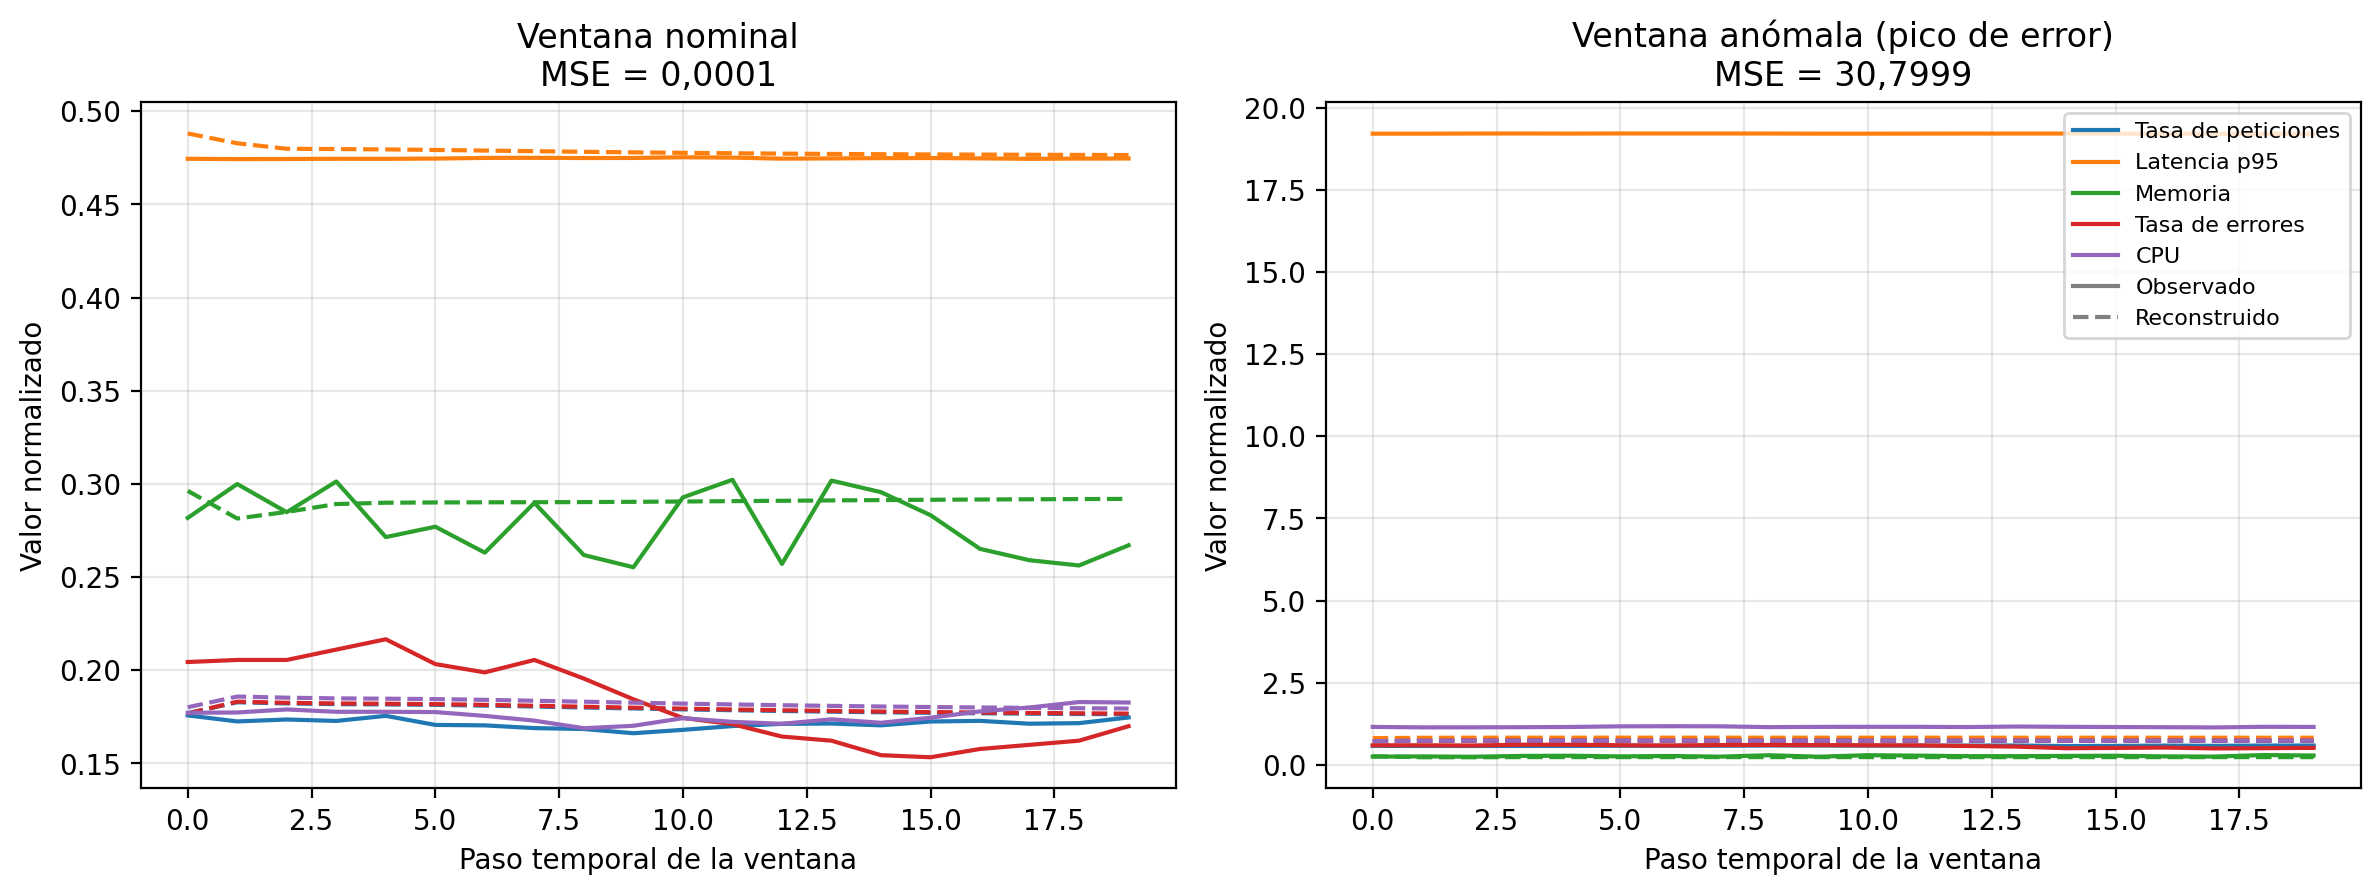
\includegraphics[width=0.95\textwidth]{./Figures/reconstruccion_ejemplo.png}
\caption{Señal observada (línea continua) y reconstruida (línea discontinua) para una ventana nominal y una ventana anómala. El eje vertical está en la escala normalizada de entrada al modelo.}
\label{fig:reconstruccion}
\end{figure}

\subsection{Desempeño de clasificación}

El conjunto de prueba comprendió 2861~ventanas, de las que 267 (un 9,3~\%) resultaron anómalas por contener al menos un instante inyectado. Con el umbral desplegado de $0{,}0025$, correspondiente al percentil 99,5 de los errores de validación, el detector clasificó correctamente 262 de las 267~ventanas anómalas y solo marcó 16 de las 2594~ventanas nominales como anómalas. La tabla~\ref{tab:metricas-resultado} reporta las métricas resultantes y la matriz de confusión se incluye en el panel inferior izquierdo de la figura~\ref{fig:eval-modelo}.

\begin{table}[htbp]
\centering
\small
\caption{Métricas de clasificación con el umbral desplegado (percentil 99,5 de validación).}
\label{tab:metricas-resultado}
\begin{tabular}{@{}l@{\hspace{3em}}r@{}}
\toprule
\textbf{Métrica} & \textbf{Valor} \\
\midrule
Exactitud & 0,993 \\
Precisión & 0,942 \\
Sensibilidad & 0,981 \\
F1-score & 0,961 \\
Tasa de falsos positivos & 0,006 \\
\bottomrule
\end{tabular}
\end{table}

La sensibilidad cercana a 0,98 indica que la mayoría de las ventanas anómalas superaron el umbral, mientras que la precisión por encima de 0,94 y la tasa de falsos positivos del 0,6~\% reflejan que las alertas se concentraron en ventanas efectivamente anómalas. El panel inferior derecho de la figura~\ref{fig:eval-modelo} compara estas métricas de forma visual.

\subsection{Sensibilidad al umbral}

El umbral es el parámetro que gobierna el compromiso entre detectar más anomalías y generar más falsas alertas. La tabla~\ref{tab:barrido-umbral} y la figura~\ref{fig:barrido-umbral} resumen un barrido en el que el umbral se recalculó como distintos percentiles del error sobre las ventanas nominales del conjunto de prueba. Percentiles bajos aumentaron la sensibilidad a costa de más falsos positivos: en el percentil 95 la precisión cayó a 0,67 con una tasa de falsos positivos del 5~\%. El percentil 99,5 ofreció el mejor compromiso, con F1-score de 0,965 y una tasa de falsos positivos del 0,5~\%. El percentil 99,9 ilustró el riesgo opuesto: un único tramo nominal con error atípicamente alto elevó el umbral de forma desproporcionada, la sensibilidad se desplomó a 0,27 y la mayoría de las anomalías quedaron sin detectar.

\begin{table}[h]
\centering
\small
\caption{Barrido del umbral sobre percentiles del error en ventanas nominales.}
\label{tab:barrido-umbral}
\begin{tabular}{@{}ccccc@{}}
\toprule
\textbf{Percentil} & \textbf{Precisión} & \textbf{Sensibilidad} & \textbf{F1-score} & \textbf{TFP} \\
\midrule
95,0  & 0,671 & 0,993 & 0,801 & 0,050 \\
97,5  & 0,802 & 0,989 & 0,886 & 0,025 \\
99,0  & 0,910 & 0,985 & 0,946 & 0,010 \\
99,5  & 0,953 & 0,978 & 0,965 & 0,005 \\
99,9  & 0,960 & 0,270 & 0,421 & 0,001 \\
\bottomrule
\end{tabular}
\end{table}

\begin{figure}[h]
\centering
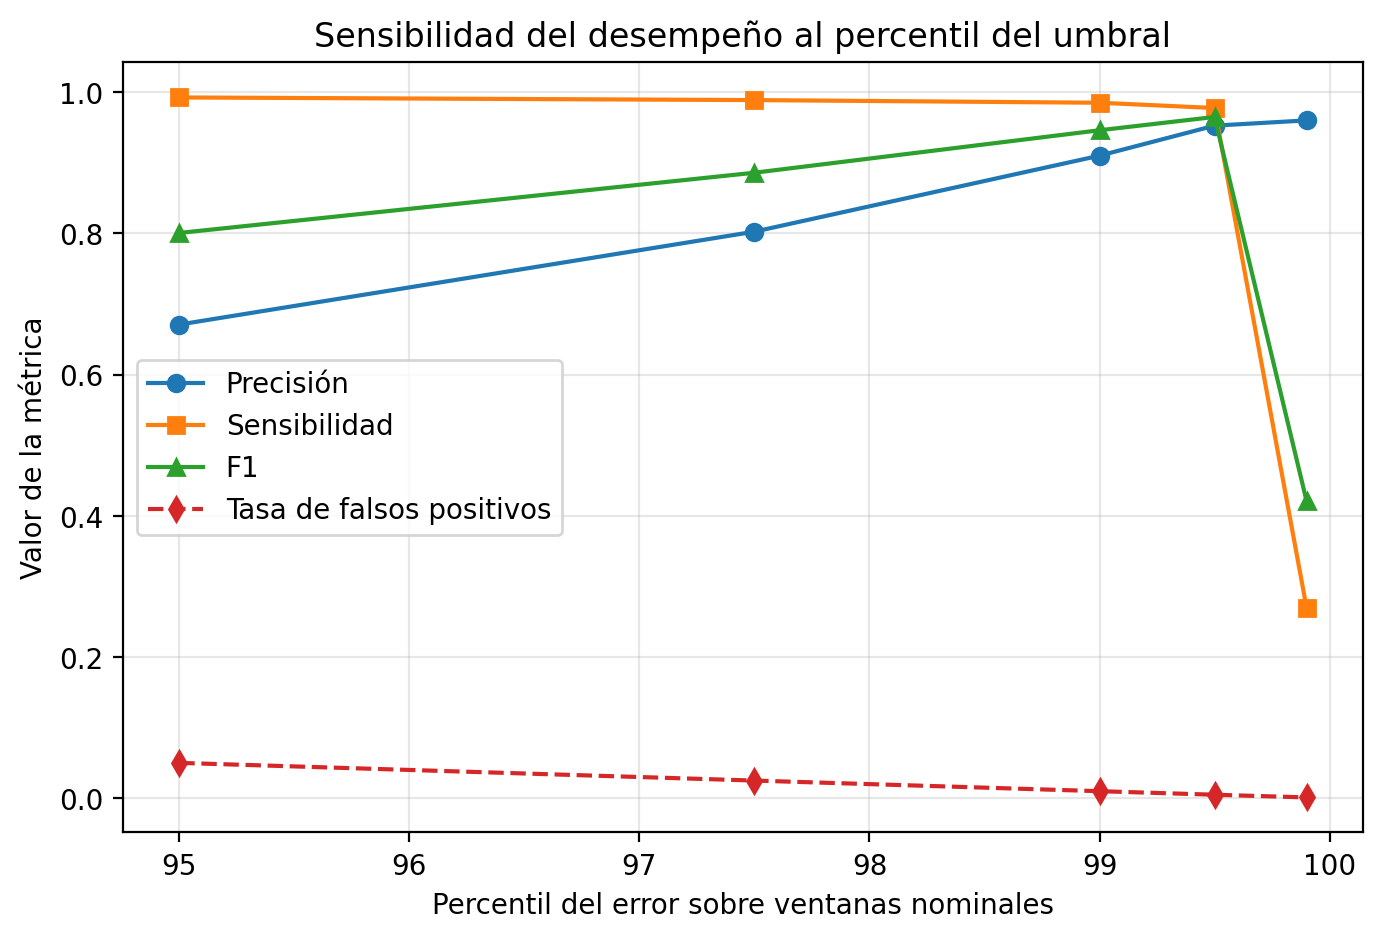
\includegraphics[width=0.80\textwidth]{./Figures/barrido_umbral.png}
\caption{Variación de precisión, sensibilidad, F1-score y tasa de falsos positivos según el percentil del error en ventanas nominales adoptado como umbral.}
\label{fig:barrido-umbral}
\end{figure}

\subsection{Comparación con una línea base de umbrales fijos}

Para situar el desempeño frente a la práctica habitual descrita en el capítulo~\ref{Chapter1}, se implementó una línea base de umbrales fijos univariados. Para cada métrica técnica se fijó un límite a partir de los percentiles extremos observados en ventanas nominales, y una ventana se marcó como anómala cuando alguna métrica superó su límite superior o cayó por debajo de su límite inferior. La tabla~\ref{tab:comparacion-baseline} contrasta ambos enfoques sobre el mismo conjunto de prueba.

\begin{table}[h]
\centering
\small
\caption{Comparación entre la línea base de umbrales fijos y el autoencoder LSTM.}
\label{tab:comparacion-baseline}
\begin{tabular}{@{}p{0.34\textwidth}cccc@{}}
\toprule
\textbf{Enfoque} & \textbf{Precisión} & \textbf{Sensibilidad} & \textbf{F1-score} & \textbf{TFP} \\
\midrule
Umbrales fijos univariados & 0,959 & 0,963 & 0,961 & 0,004 \\
Autoencoder LSTM & 0,942 & 0,981 & 0,961 & 0,006 \\
\bottomrule
\end{tabular}
\end{table}

Las anomalías inyectadas en el ensayo son deliberadamente marcadas, de modo que ambos enfoques las detectaron en buena medida y obtuvieron un F1-score equivalente. El autoencoder logró mayor sensibilidad, mientras que la línea base alcanzó algo más de precisión y una tasa de falsos positivos ligeramente menor sobre este conjunto. Este resultado es esperable: cuando una anomalía empuja una sola métrica a un valor extremo, un umbral univariado basta para detectarla.

La ventaja del modelo no reside, por tanto, en superar a la línea base sobre anomalías evidentes, sino en dos aspectos discutidos en el capítulo~\ref{Chapter1}. En primer lugar, la línea base requiere fijar y mantener un límite por cada métrica, mientras que el autoencoder concentra la decisión en un único umbral calibrado sobre el error de reconstrucción. En segundo lugar, el modelo procesa las once variables de forma conjunta y aprende el patrón circadiano del servicio; así puede distinguir una caída de tráfico esperable en la madrugada de una caída anómala en horario pico, distinción que un umbral fijo por métrica no captura sin reglas adicionales por franja horaria.

\subsection{Latencia de detección}

Además de clasificar correctamente las ventanas, resulta relevante evaluar la rapidez con que reacciona el detector una vez iniciada una anomalía. La tabla~\ref{tab:latencia-deteccion} resume, por tipo de anomalía inyectada, la cantidad de ventanas afectadas, las detectadas y el retardo entre la primera ventana afectada y la primera detección, medido en ventanas de inferencia (una cada 30~segundos). Los picos de latencia y de memoria se detectaron en la primera ventana que los contuvo, sin retardo apreciable, porque elevaron el error de reconstrucción de inmediato. La caída de tráfico requirió alrededor de cinco ventanas, equivalentes a unos 2,5~minutos, hasta que el descenso de demanda se acumuló lo suficiente en la ventana para superar el umbral. Ese retardo es coherente con su menor amplitud y con los falsos negativos analizados en la sección~\ref{sec:analisis-errores}.

\begin{table}[h]
\centering
\small
\caption{Latencia de detección por tipo de anomalía inyectada.}
\label{tab:latencia-deteccion}
\begin{tabular}{@{}>{\raggedright\arraybackslash}p{0.22\textwidth}cccc@{}}
\toprule
\textbf{Anomalía} & \textbf{Vent.} & \textbf{Detect.} & \textbf{Retardo (vent.)} & \textbf{Retardo aprox.} \\
\midrule
Pico de latencia & 79 & 79 & 0 & inmediato \\
Caída de tráfico & 49 & 44 & 5 & 2,5~min \\
Pico de memoria & 139 & 139 & 0 & inmediato \\
\bottomrule
\end{tabular}
\end{table}

%----------------------------------------------------------------------------------------
%	SECTION 3
%----------------------------------------------------------------------------------------

\section{Análisis de errores}
\label{sec:analisis-errores}

El análisis de los casos en que el detector falla es tan relevante como las métricas agregadas, porque revela los límites del enfoque y orienta la operación. Sobre el conjunto de prueba, los errores se concentraron en dos categorías de baja frecuencia: 5 falsos negativos (ventanas anómalas no detectadas) y 16 falsos positivos (ventanas nominales marcadas como anómalas).

\subsection{Falsos negativos}

Los 5 falsos negativos pertenecieron en su totalidad al tramo de caída de tráfico, del que se detectaron 44 de las 49 ventanas afectadas; los picos de latencia y de memoria se detectaron por completo. La caída de tráfico fue el tipo que menos elevó el error de reconstrucción: a diferencia de un pico de latencia o de memoria, que empuja una variable hacia valores altos poco frecuentes, una caída reduce la tasa de peticiones hacia valores que el modelo también observa en horarios de baja demanda. En el panel de línea de tiempo de la figura~\ref{fig:eval-modelo} se aprecia que el tramo de caída de tráfico apenas supera el umbral, frente al pico de latencia, con un error varios órdenes de magnitud mayor.

Las ventanas no detectadas se ubicaron en los bordes del tramo, donde una ventana deslizante de 20 pasos contiene solo uno o dos instantes anómalos y promedia mayormente comportamiento nominal. Este efecto es coherente con la decisión de diseño de la sección~\ref{sec:pipeline-datos}: una longitud de 20 pasos diluye perturbaciones de un único muestreo y privilegia la detección de desvíos sostenidos sobre los puntuales.

\subsection{Falsos positivos}

Los 16 falsos positivos se concentraron en ventanas de transición que combinan el final de un tramo nominal con el comienzo de una anomalía. La agregación \texttt{rate(...[5m])} suavizaba cada métrica sobre una ventana de cinco minutos; por ello, un instante todavía etiquetado como nominal e inmediatamente anterior a un tramo anómalo ya incorporaba parte de la perturbación y producía un error elevado. A ello se sumó alguna ventana nominal aislada con ruido de alta frecuencia. En operación, estos casos límite se mitigaron con los mecanismos descritos en la sección~\ref{sec:integracion}: el filtrado por confianza mínima descartó excesos marginales sobre el umbral y la confirmación por dos ciclos consecutivos evitó abrir alertas ante un único ciclo transitorio.

\subsection{Contribución de cada variable al error}

El error de reconstrucción agrega las once variables de la ventana, pero no todas contribuyen por igual ante una anomalía. La tabla~\ref{tab:error-por-variable} compara, para las cinco métricas técnicas, el error mediano en ventanas nominales con el error medio en ventanas anómalas. En régimen nominal todas las variables se reconstruyeron con error muy bajo. Ante anomalías, la latencia percentil 95 dominó ampliamente el error, con un valor varios órdenes de magnitud superior al del resto de las métricas, reflejo de que el pico de latencia fue la perturbación más extrema del ensayo. Las variables temporales derivadas se reconstruyeron con error reducido en ambos regímenes, lo que confirma que aportan contexto estable sobre el momento del día sin introducir ruido en la señal de anomalía.

\begin{table}[h]
\centering
\small
\caption{Error de reconstrucción por variable técnica: mediana en ventanas nominales y media en ventanas anómalas.}
\label{tab:error-por-variable}
\begin{tabular}{@{}p{0.28\textwidth}rr@{}}
\toprule
\textbf{Variable} & \textbf{Nominal (mediana)} & \textbf{Anómala (media)} \\
\midrule
\texttt{request\_rate} & 0{,}000076 & 0{,}049 \\
\texttt{latency\_p95} & 0{,}000024 & 81{,}3 \\
\texttt{memory\_usage} & 0{,}000270 & 0{,}47 \\
\texttt{error\_rate} & 0{,}00039 & 0{,}050 \\
\texttt{cpu\_usage} & 0{,}000077 & 0{,}076 \\
\bottomrule
\end{tabular}
\\[0.5em]
{\footnotesize Nota: error cuadrático medio normalizado por variable.}
\end{table}

\subsection{Errores observados en el despliegue real}

El análisis de errores no se limitó al conjunto sintético. Durante la validación sobre la infraestructura autorizada surgieron patrones de error que motivaron decisiones de diseño documentadas a lo largo de la memoria, sin exponer las series confidenciales involucradas.

El caso más relevante fue una tasa elevada de falsos positivos al evaluar sobre Prometheus un modelo entrenado con un escalador adaptativo. Las series productivas, con distinta escala absoluta, quedaron desplazadas respecto del dominio aprendido y el error superó el umbral de forma sistemática sobre tramos nominales. La adopción del escalado \texttt{fixed\_minmax}, junto con la reducción del stride a uno, eliminó ese desajuste, como se detalló en la sección~\ref{sec:entrenamiento}.

Un segundo patrón provino de la agregación de métricas multiserie: la latencia percentil 95 se calculaba sumando las series por extremo en lugar de tomar el máximo; ello inflaba el valor varias veces y producía detecciones espurias. La corrección de la semántica de agregación, resumida en la tabla~\ref{tab:promql-queries}, alineó los valores con los del panel de Grafana.

Un tercer patrón apareció tras pausas del entorno: cuando Prometheus presentaba un hueco de recolección, la ventana de inferencia quedaba incompleta y el relleno con ceros generaba una secuencia artificial que el modelo marcaba como anómala. La salvaguarda de disponibilidad de datos, que exige una ventana completa y reciente antes de puntuar, y la confirmación por ciclos consecutivos eliminaron esas alertas transitorias. Estos hallazgos confirmaron que, en un sistema de detección no supervisado, una fracción importante de los errores no proviene del modelo en sí, sino de discrepancias entre el dato de entrenamiento y el dato de inferencia.

%----------------------------------------------------------------------------------------
%	SECTION 4
%----------------------------------------------------------------------------------------

\section{Ensayos de integración del sistema}
\label{sec:ensayos-integracion}

Más allá del desempeño del modelo aislado, se verificó el comportamiento del sistema completo en condiciones cercanas a las de uso. Los ensayos de integración se realizaron sobre el entorno demostrativo orquestado con Docker Compose, que reúne el servicio simulado, Prometheus, Grafana y el contenedor de detección descritos en la sección~\ref{sec:integracion}.

\subsection{Detección extremo a extremo}

El servicio simulado ofreció un punto de entrada para inyectar anomalías en tiempo real, lo que permitió ejercitar el bucle completo: recolección desde Prometheus, preprocesamiento, inferencia, comparación con el umbral, deduplicación y emisión de alertas. Para cada tipo de anomalía se inyectó un episodio y se verificó la cadena de respuesta. La tabla~\ref{tab:integracion-escenarios} resume los escenarios ejecutados.

\begin{table}[h]
\centering
\small
\caption{Escenarios de integración ejercitados en el entorno demostrativo.}
\label{tab:integracion-escenarios}
\begin{tabular}{@{}>{\raggedright\arraybackslash}p{0.22\textwidth}>{\raggedright\arraybackslash}p{0.30\textwidth}cc@{}}
\toprule
\textbf{Escenario} & \textbf{Métrica afectada} & \textbf{Detección} & \textbf{Alerta} \\
\midrule
Pico de latencia & Latencia percentil 95 & Sí & Sí \\
Ráfaga de errores & Tasa de errores & Sí & Sí \\
Pico de memoria & Memoria residente & Sí & Sí \\
Caída de tráfico & Tasa de peticiones & Sí & Sí \\
Tráfico nominal & --- & No & No \\
\bottomrule
\end{tabular}
\end{table}

En todos los escenarios con anomalía inyectada el sistema generó la detección y la alerta correspondiente una vez que la ventana de inferencia acumuló datos anómalos suficientes; en el escenario de tráfico nominal no se emitieron alertas.

\subsection{Canal de alertas intercambiable}

La integración con Opsgenie descrita en la sección~\ref{sec:integracion} se implementó como un adaptador HTTP desacoplado del núcleo de detección. El servicio de inferencia seleccionó el canal de notificación mediante el parámetro \path{alerting.provider} de \path{config/alerting.yaml}, de modo que el mismo flujo de confirmación, deduplicación y resolución operó con distintos backends sin modificar la lógica de puntuación.

Durante los ensayos de integración del entorno demostrativo se utilizó Jira Service Management (JSM) Operations como canal de alertas. Atlassian retiró Opsgenie para nuevos clientes y migró la gestión de incidentes a JSM; el \textit{endpoint} de integración de Operations conserva compatibilidad con el esquema y la autenticación \texttt{GenieKey} de Opsgenie. El cliente \path{JSMClient} extendió \path{OpsgenieClient} y solo cambiaba la URL base y el \texttt{alias} estable por anomalía, que permitía cerrar la misma alerta con el endpoint \texttt{close-by-alias}. En producción el sistema siguió emitiendo alertas hacia Opsgenie; en la demo reproducible se configuró \path{provider: jsm} para validar el flujo completo sobre la plataforma sucesora sin alterar el diseño documentado en capítulos anteriores.

\subsection{Demostración en el entorno demostrativo}

Para documentar el comportamiento extremo a extremo se ejecutó una demostración en vivo sobre el stack Docker Compose. Tras acumular tráfico nominal en Prometheus, se inyectó un pico sostenido de latencia mediante \texttt{POST /anomaly} al servicio simulado. El detector consultó las métricas, reconstruyó la ventana deslizante y, tras dos ciclos consecutivos por encima del umbral, registró la apertura de anomalía y envió la alerta a JSM Operations.

La figura~\ref{fig:demo-grafana} muestra el panel de Grafana durante el episodio: la latencia percentil 95 se elevó a unos 9--10~s mientras el resto de las métricas permaneció en régimen nominal y el servicio continuó reportándose como activo. Esa discrepancia univariada dentro de un contexto multivariado nominal es precisamente la señal que el autoencoder traduce en un error de reconstrucción elevado.

\begin{figure}[htbp]
\centering
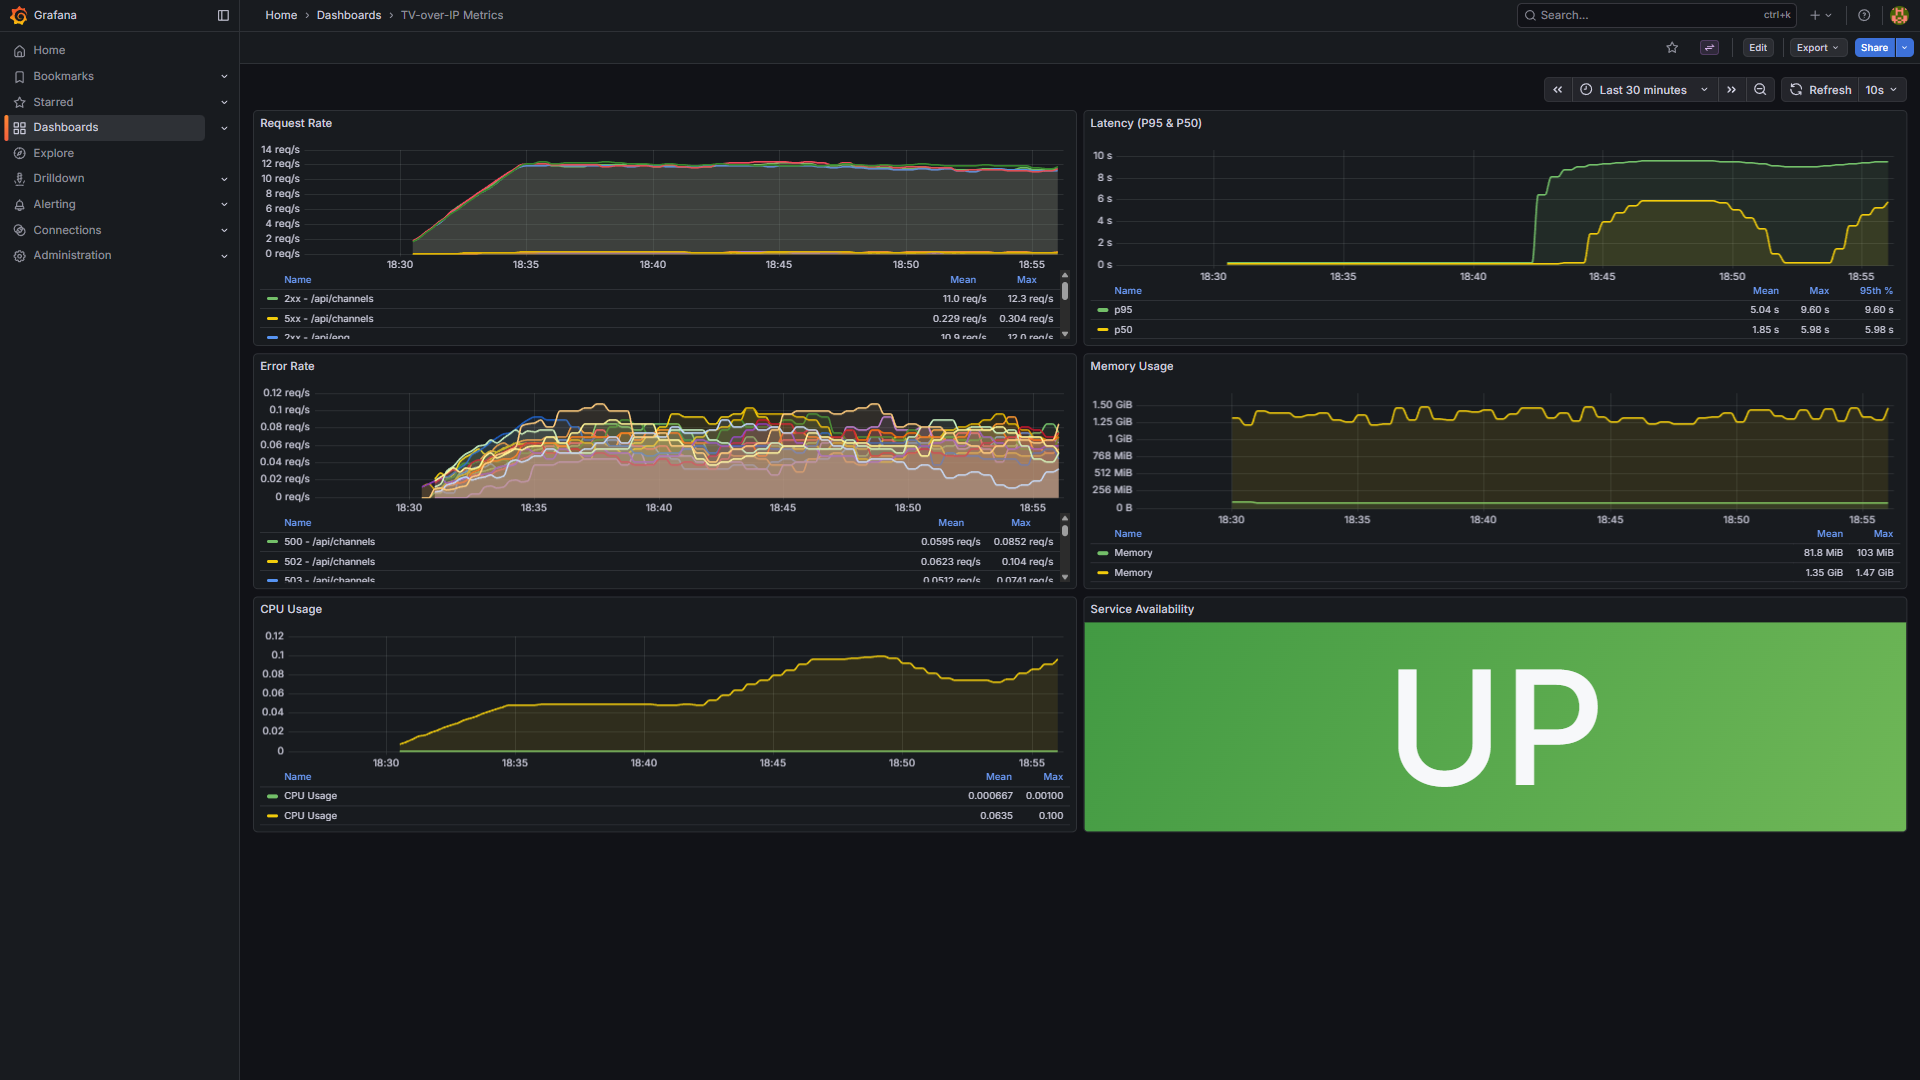
\includegraphics[width=\textwidth]{./Figures/demo_grafana.png}
\caption{Panel de Grafana durante la demostración en vivo: pico sostenido de latencia percentil 95 con el resto de métricas nominales.}
\label{fig:demo-grafana}
\end{figure}

La figura~\ref{fig:demo-logs} reproduce el extracto de registros del detector para el mismo incidente. Se observa la secuencia completa: detección potencial en el primer ciclo, confirmación como \texttt{NEW ANOMALY} en el segundo, envío de la alerta a JSM, registros periódicos de deduplicación (\textit{heartbeat}) mientras la anomalía persistió, escalamiento a los 30~minutos y cierre automático cuando las métricas se normalizaron.

\begin{figure}[htbp]
\centering
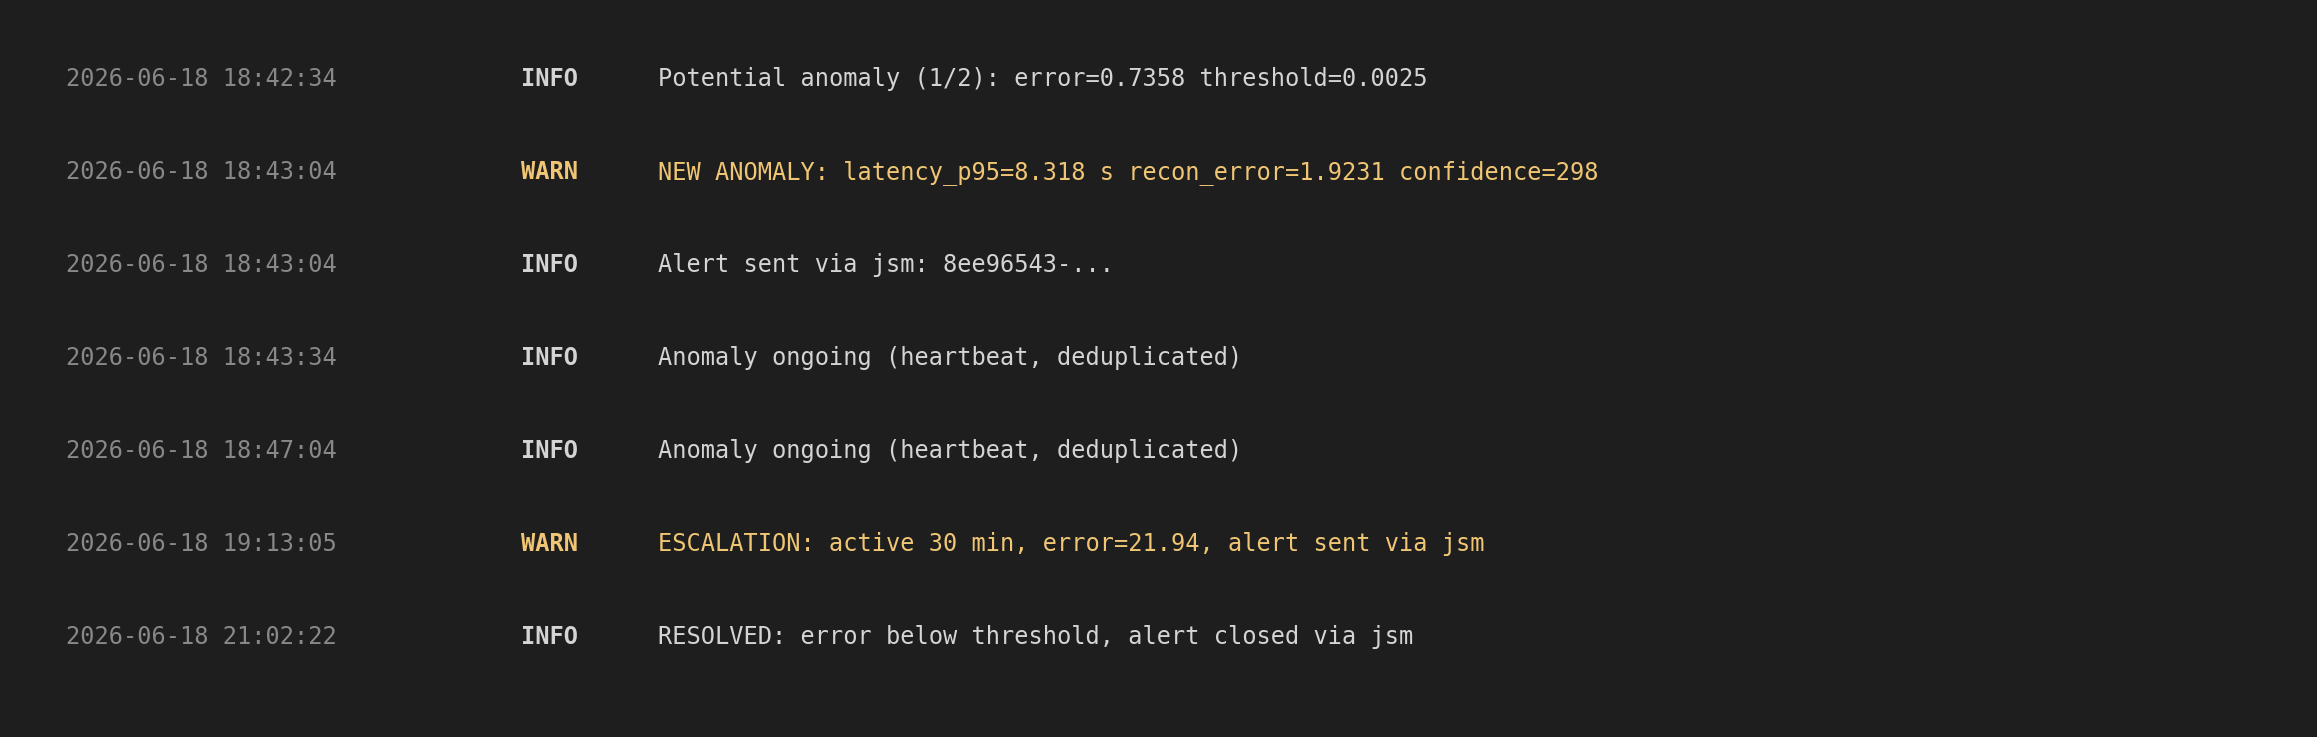
\includegraphics[width=\textwidth]{./Figures/demo_logs.png}
\caption{Extracto de registros del detector durante la demostración: apertura, deduplicación, escalamiento y resolución.}
\label{fig:demo-logs}
\end{figure}

En JSM Operations la alerta de apertura apareció con prioridad P3, el error de reconstrucción, la confianza, la comparación métrica observada vs.\ reconstruida y un enlace contextual al panel de Grafana acotado al intervalo de la anomalía (panel izquierdo de la figura~\ref{fig:demo-jsm}). La integración \texttt{autoencoder-alerting (API)} identificó el origen del payload HTTP. Tras 30~minutos de persistencia, el mecanismo de escalamiento generó una segunda notificación de prioridad P2 con la duración acumulada y el error vigente (panel derecho). Tras eliminar la anomalía inyectada, el detector cerró la alerta en JSM con una nota de resolución que incluyó la duración del incidente.

\begin{figure}[htbp]
\centering
\begin{minipage}{0.48\textwidth}
\centering
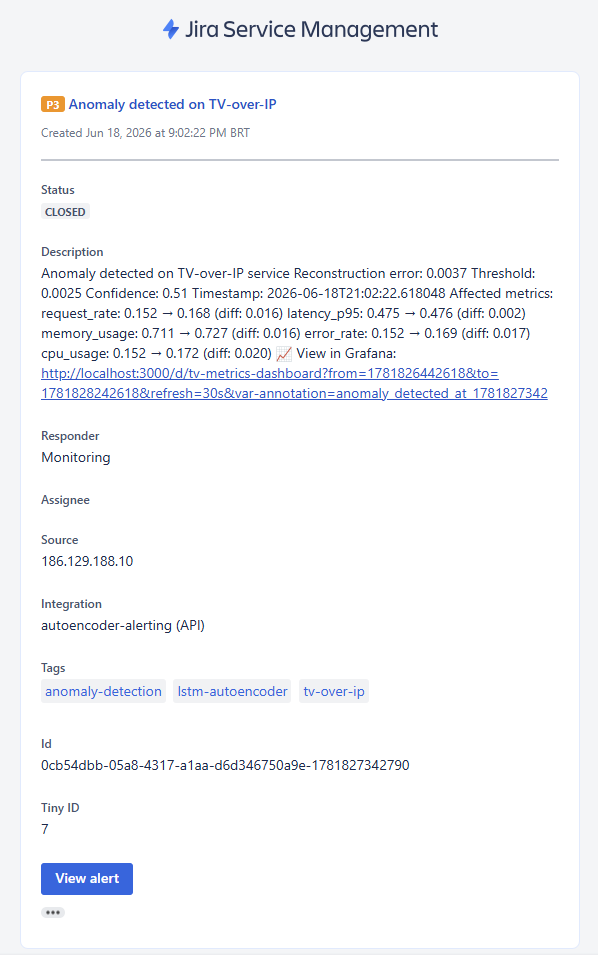
\includegraphics[width=\textwidth]{./Figures/demo_jsm_alerta.png}\\[0.3em]
{\small (a) Alerta de apertura}
\end{minipage}\hfill
\begin{minipage}{0.48\textwidth}
\centering
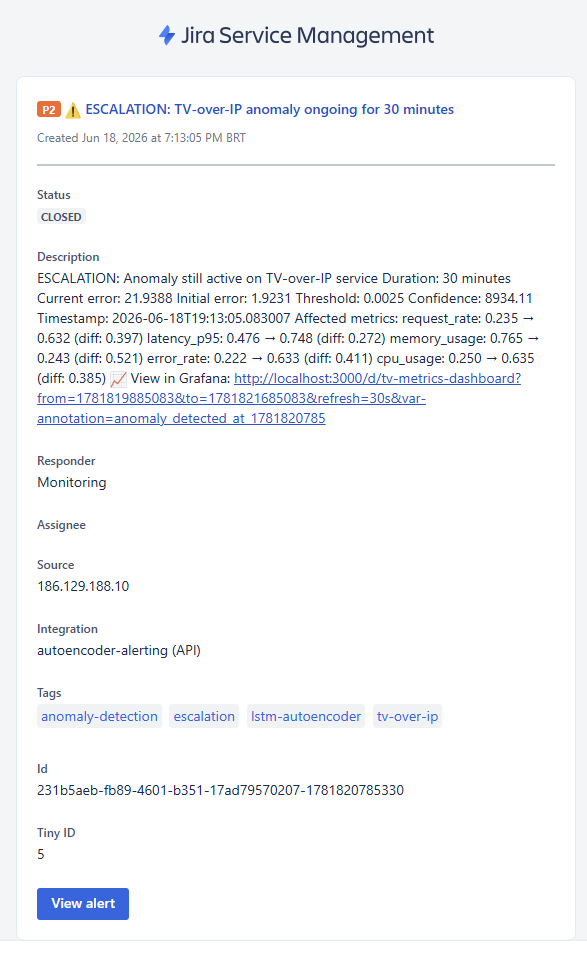
\includegraphics[width=\textwidth]{./Figures/demo_jsm_escalacion.png}\\[0.3em]
{\small (b) Escalamiento a los 30~min}
\end{minipage}
\caption{Alertas en Jira Service Management Operations durante la demostración en vivo: apertura con contexto de detección y escalamiento por persistencia.}
\label{fig:demo-jsm}
\end{figure}

\subsection{Deduplicación de alertas}

Un objetivo operativo central, derivado del problema de fatiga de alertas planteado en el capítulo~\ref{Chapter1}, fue evitar la repetición de notificaciones durante un mismo incidente. Sin deduplicación, una anomalía sostenida generaba una alerta en cada ciclo de 30~segundos. Con el mecanismo de seguimiento por identificador único, confirmación por ciclos y notificación de resolución, cada incidente produjo una única alerta de apertura y una de cierre. La figura~\ref{fig:ciclo-vida-alerta} resume la máquina de estados implementada; la tabla~\ref{tab:deduplicacion} contrasta ambos comportamientos sobre un episodio sostenido.

\begin{figure}[htbp]
\centering
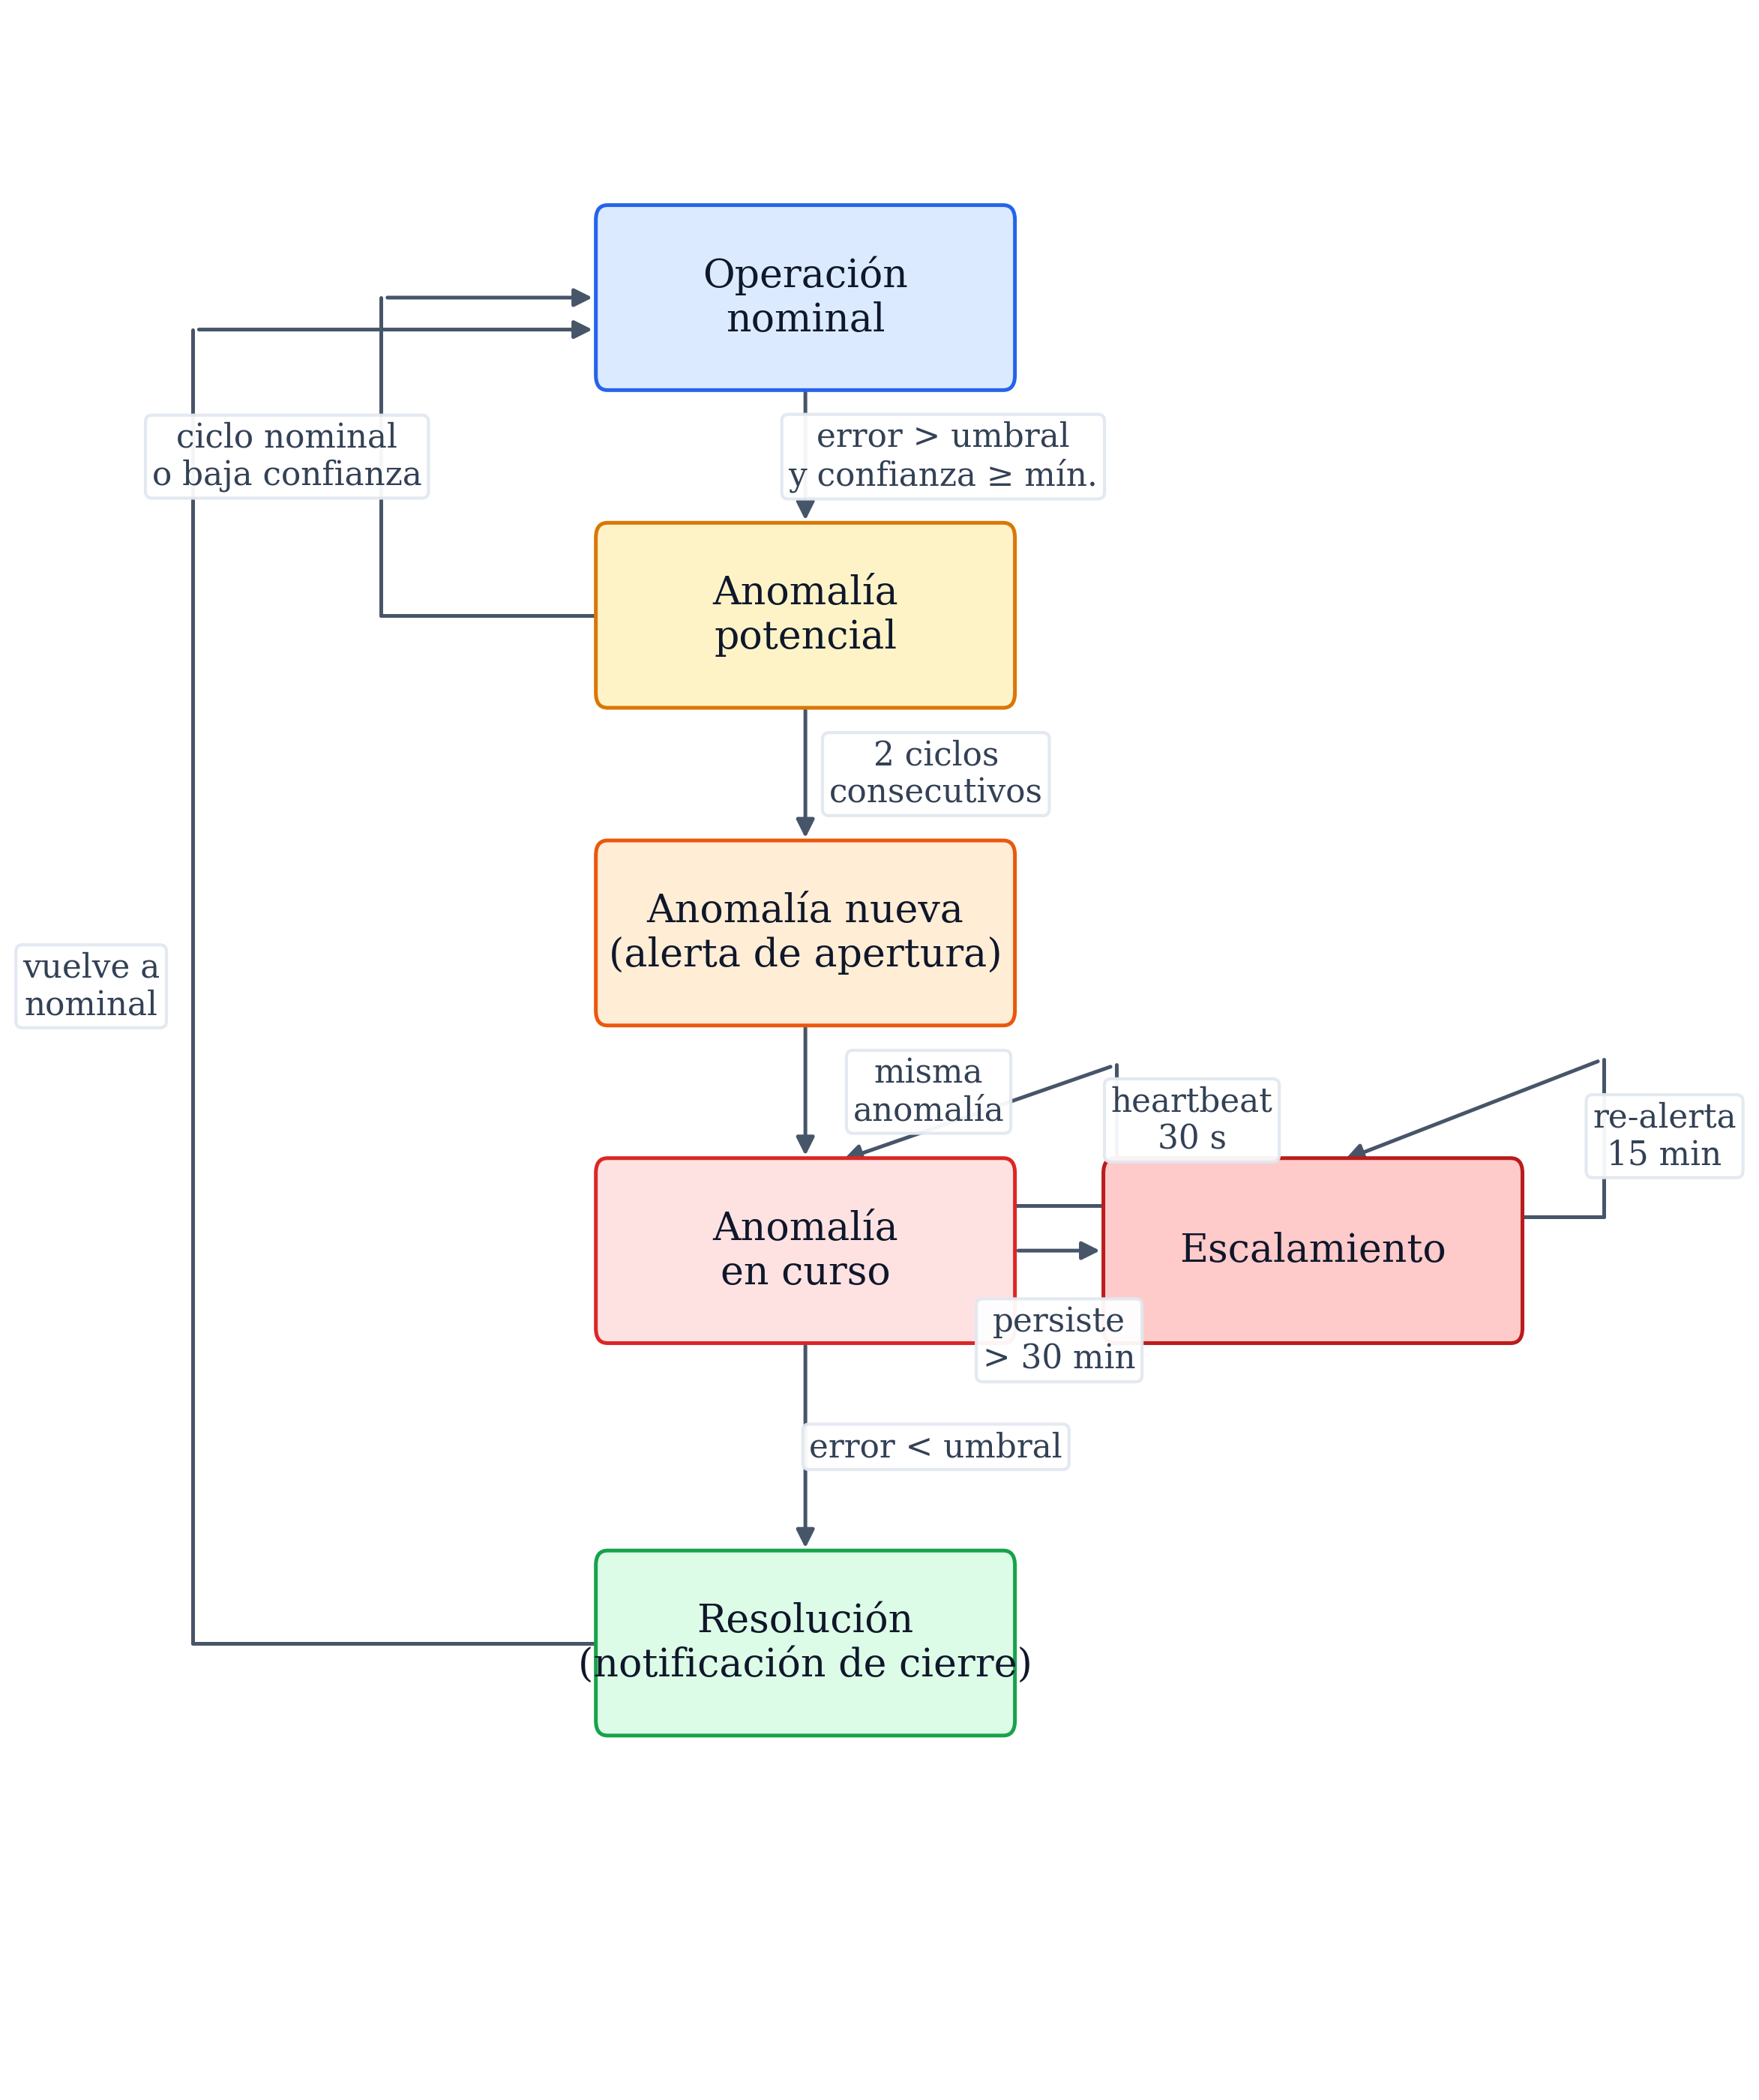
\includegraphics[width=\textwidth]{./Figures/ciclo_vida_alerta.png}
\caption{Ciclo de vida de una alerta: transiciones entre operación nominal, confirmación, deduplicación, escalamiento y resolución.}
\label{fig:ciclo-vida-alerta}
\end{figure}

\begin{table}[h]
\centering
\small
\caption{Efecto de la deduplicación sobre un incidente sostenido.}
\label{tab:deduplicacion}
\begin{tabular}{@{}p{0.40\textwidth}cc@{}}
\toprule
\textbf{Comportamiento} & \textbf{Sin deduplicación} & \textbf{Con deduplicación} \\
\midrule
Alertas por incidente & 12 o más & 1 (más resolución) \\
Notificación de resolución & No & Sí \\
Confirmación previa & No & 2 ciclos \\
\bottomrule
\end{tabular}
\end{table}

\subsection{Costo de inferencia y robustez}

El costo de cómputo se mantuvo dentro de los límites previstos. Cada ciclo de detección, que comprende la consulta a Prometheus, el preprocesamiento, la reconstrucción y la comparación con el umbral, se completó en menos de un segundo dentro del contenedor con una CPU virtual, holgadamente por debajo del intervalo de 30~segundos entre ciclos. El uso de memoria se mantuvo por debajo del límite asignado de 2~GB.

La robustez ante datos incompletos se verificó suspendiendo y reanudando el entorno: tras un hueco de recolección, el detector omitió los ciclos cuya ventana no alcanzaba el tamaño requerido o presentaba muestras antiguas, y reanudó la puntuación una vez que dispuso de una ventana completa, sin emitir falsas alertas por relleno con ceros. Este comportamiento, junto con la continuidad del servicio ante errores puntuales de consulta, confirmó que el sistema sostuvo el monitoreo de forma estable en condiciones de operación realistas.
